\documentclass[DIN, pagenumber=false, fontsize=11pt, parskip=half]{scrartcl}

\usepackage{amsmath}
\usepackage{amsfonts}
\usepackage{amssymb}
\usepackage{enumitem}
\usepackage[utf8]{inputenc} 
\usepackage[ngerman]{babel} 
\usepackage[T1]{fontenc} 
\usepackage{pgfplots}
\usepackage{xcolor}
\usepackage{listings}
\usepackage{float}
\usepackage{graphicx}
\usepackage{booktabs}
\usepackage{tkz-euclide}
\usepackage{svg}
\usepackage{trfsigns}
\usepackage{mathtools}

\DeclarePairedDelimiter\abs{\lvert}{\rvert}%
\DeclarePairedDelimiter\norm{\lVert}{\rVert}%

\definecolor{mygreen}{RGB}{28,172,0} % color values Red, Green, Blue
\definecolor{mylilas}{RGB}{170,55,241}

\tikzstyle{neuron}=[circle,fill=black!25,minimum size=30pt,inner sep=0pt]

\lstset{language=Matlab,%
    %basicstyle=\color{red},
    breaklines=true,%
    morekeywords={matlab2tikz},
    keywordstyle=\color{blue},%
    morekeywords=[2]{1}, keywordstyle=[2]{\color{black}},
    identifierstyle=\color{black},%
    stringstyle=\color{mylilas},
    commentstyle=\color{mygreen},%
    showstringspaces=false,%without this there will be a symbol in the places where there is a space
    numbers=left,%
    numberstyle={\tiny \color{black}},% size of the numbers
    numbersep=9pt, % this defines how far the numbers are from the text
    emph=[1]{for,end,break},emphstyle=[1]\color{red}, %some words to emphasise
    %emph=[2]{word1,word2}, emphstyle=[2]{style},    
}

\title{Einführung in die Neuroinformatik}
\author{Tim Luchterhand, Paul Nykiel (Gruppe P)}

\begin{document}
    \maketitle
    \section{Dropout}
    \subsection{}
    \begin{enumerate}[label=\alph*)]
        \item Durch Dropout wird die Relevanz einzelner Neuronen reduziert, da das trainiert Netzwerk auch nur mit einer Teilmenge aller Neuronen
            funktioniert. Es werden quasi mehrere Netze mit weniger Neuronen trainiert und dann der Durchschnitt verwendet. Im Gegensatz zur naiven Implementierung
            mit mehreren Netzten wird allerdings deutlich weniger Rechenkapazität benötigt.
        \item Die Gewichte müssen mit dem Faktor $1 - p = \frac{2}{3}$ skaliert werden.
    \end{enumerate}

    \subsection{}
    \begin{enumerate}[label=\alph*)]
        \item $ $ \lstinputlisting{networkDropout.m}
        \item $ $ \lstinputlisting[lastline=3]{b10a01.m}
        \item $ $ \lstinputlisting[firstline=5, firstnumber=5, lastline=6]{b10a01.m}
        \item $ $ \lstinputlisting[firstline=8, firstnumber=8, lastline=10]{b10a01.m}
        \item $ $ \lstinputlisting[firstline=12, firstnumber=12, lastline=21]{b10a01.m}
            \begin{figure}[H]
                \centering
                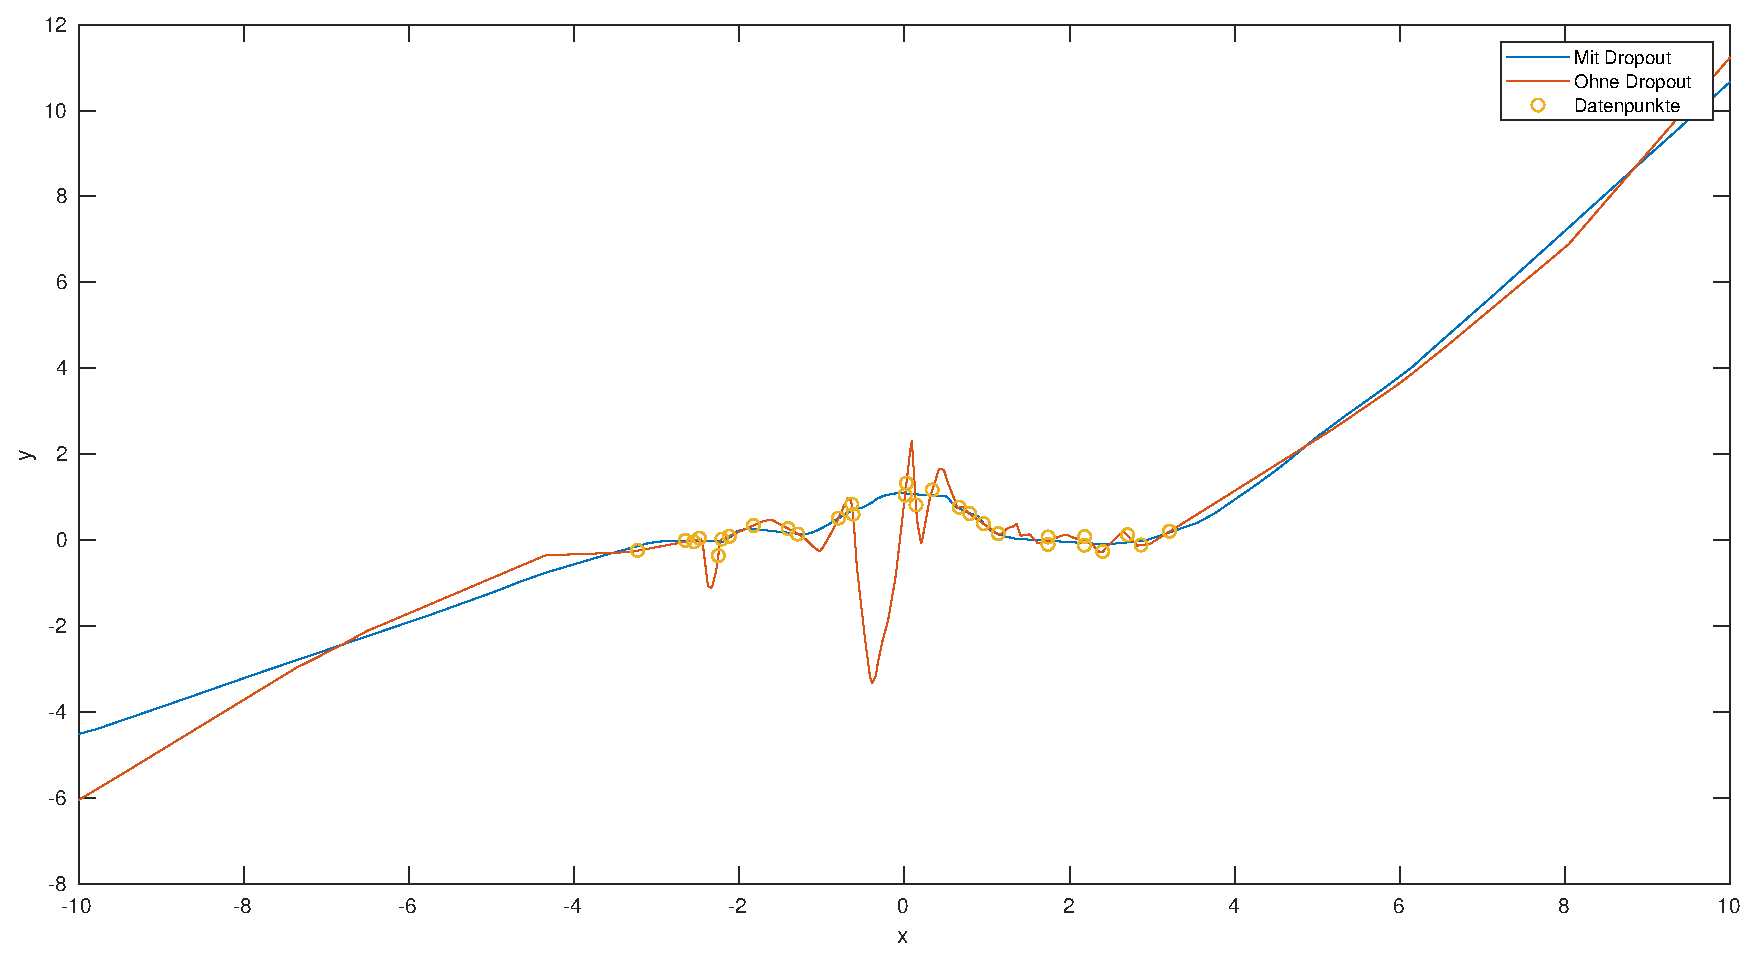
\includegraphics[width=\textwidth]{b10a01.eps}
                \caption{Ausgabe des Matlab-Skripts}
            \end{figure}
        \item $ $ \lstinputlisting[firstline=23, firstnumber=23, lastline=24]{b10a01.m}
    \end{enumerate}

    \section{Uncertainty via Dropout}
    \subsection{}
    \lstinputlisting[lastline=6]{b10a02.m}
\end{document}
